%!TEX encoding = UTF-8 Unicode
\documentclass[12pt]{article} 
\usepackage[left=0.75in,top=0.7in,right=0.75in,bottom=0.3in]{geometry} % Document margins
\usepackage{CJK}
\usepackage{graphicx}
\usepackage{mathtools}
\usepackage{mathrsfs}
\usepackage{amssymb}
\usepackage{hyperref}
\usepackage{sidecap}
\usepackage{makecell}

\makeatletter
\renewenvironment{itemize}
{\list{$\bullet$}{\leftmargin\z@ \labelwidth\z@ \itemindent-\leftmargin
\let\makelabel\descriptionlabel}}
{\endlist}
\makeatother

\begin{CJK}{UTF8}{bsmi}
\title{\textbf{Homework06 / Restricted Boltzmann Machine with Contrastive Divergence}}
\author{\textbf{李豪韋 (HW-Lee) ID 103061527}}
\date{}

\begin{document}
\vspace*{-60pt}
    {\let\newpage\relax\maketitle}

\section*{Overview}
\vspace{-20pt}
\noindent\makebox[\linewidth]{\rule{\textwidth}{0.4pt}}
\vspace{5pt}

Restricted Boltzmann Machine is a system that is able to learn data without knowing their corresponding labels, so it is used for pre-training, which is a kind of unsupervised learning to make the features easier to be found by classifiers. In this project, I tried to teach a RBM system with hand-written digits and verify its feasibility in pre-training. In Boltzmann Machine, the objective is to maximize the sum of log-likelihood of training instances, to reconstruct a testing instance so that the reconstructed instance is more 'similar' to training instances than before. Optimistically, the reconstructed input will be more robust to be classified and the variance within a class will be decreased. Finally, my system seems to successfully learn some features after feeding lots of instances, but the final weights look very different from those shown in Hinton's slides.

The more detailed information of the code is publicly available on \href{https://github.com/HW-Lee/2015-NN-Homeworks/tree/master/HW06}{$\mathsf{https://github.com/HW}$-$\mathsf{Lee/2015}$-$\mathsf{NN}$-$\mathsf{Homeworks/tree/master/HW06}$}.

\section*{Implementation}
\vspace{-20pt}
\noindent\makebox[\linewidth]{\rule{\textwidth}{0.4pt}}

\begin{enumerate}
	\item {\bf System Structure}
	\begin{figure}[ht]
		\hspace{-1em}
		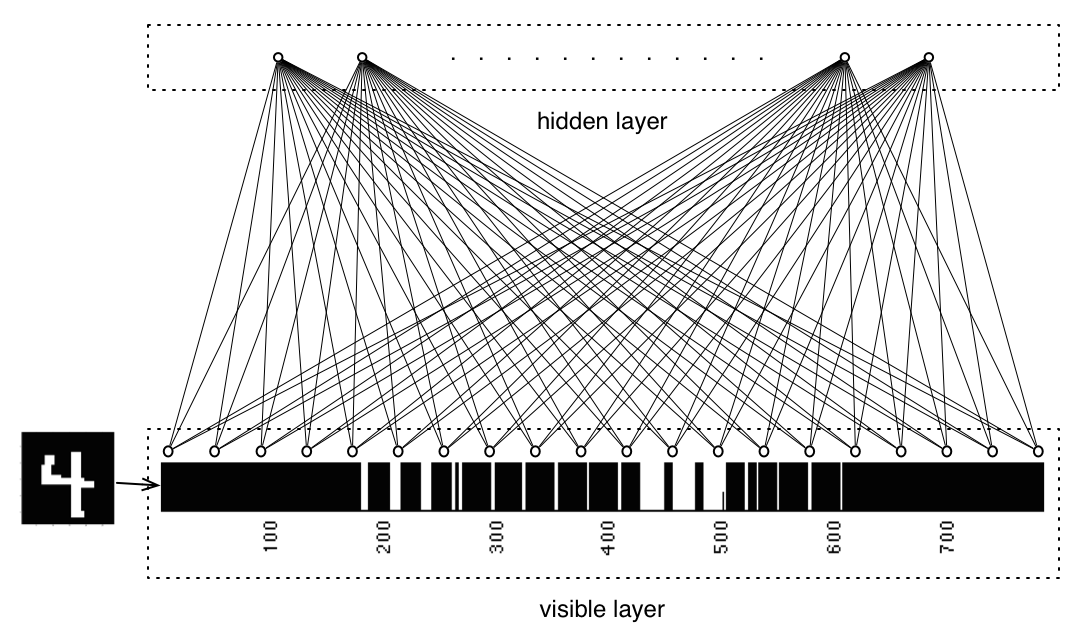
\includegraphics[scale=.45]{../res/netStruct.png}
		\caption{The net consists of $28 \times 28$ visible neurons and $450$ hidden neurons}
	\end{figure}
	
	\newpage
	\item {\bf Algorithm}
	\begin{figure}[ht]
		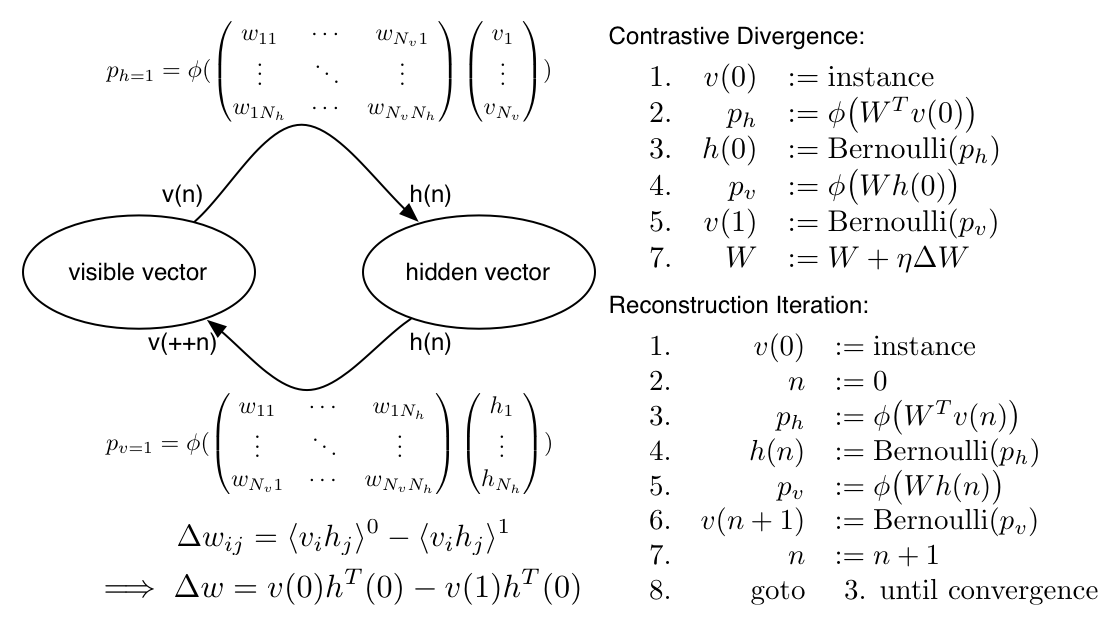
\includegraphics[scale=.4]{../res/algo.png}
		\caption{Training and reconstruction algorithm}
	\end{figure}
\end{enumerate}

\section*{Results}
\vspace{-20pt}
\noindent\makebox[\linewidth]{\rule{\textwidth}{0.4pt}}

\begin{figure}[ht]
	\begin{center}
		Successfully Reconstructed Result: with digit-7
	\end{center}
	\begin{minipage}[c]{0.55\linewidth}
	\centering
	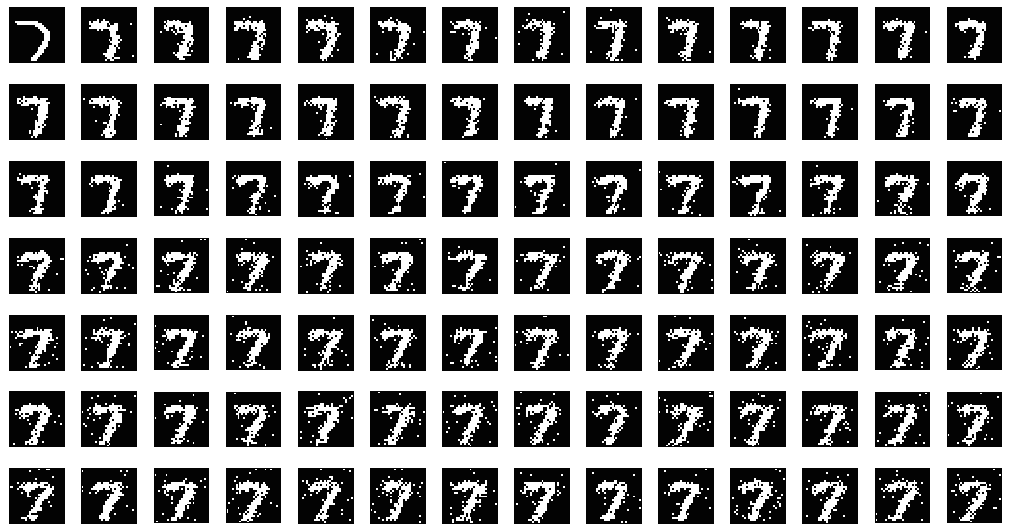
\includegraphics[scale=.3]{../res/chgVisible1.png}
	\caption{The visible neurons at each iteration, (left-to-right, top-to-bottom)}
	\end{minipage}
	\hspace{4em}
	\begin{minipage}[c]{0.35\linewidth}
	\centering
	\vspace{-1em}
	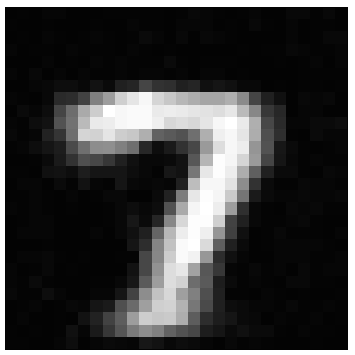
\includegraphics[scale=.45]{../res/avgVisible1.png}
	\caption{Averaged visible neurons}
	\end{minipage}
\end{figure}

\begin{center}
	The results are publicly available on \href{https://github.com/HW-Lee/2015-NN-Homeworks/tree/master/HW06/res}{$\mathsf{https://github.com/HW}$-$\mathsf{Lee/2015}$-$\mathsf{NN}$-$\mathsf{Homeworks/tree/master/HW06/res}$}.
\end{center}

\newpage
\begin{figure}[ht]
	\begin{center}
		Unsuccessfully Reconstructed Result: with digit-6
	\end{center}
	\begin{minipage}[c]{0.55\linewidth}
	\centering
	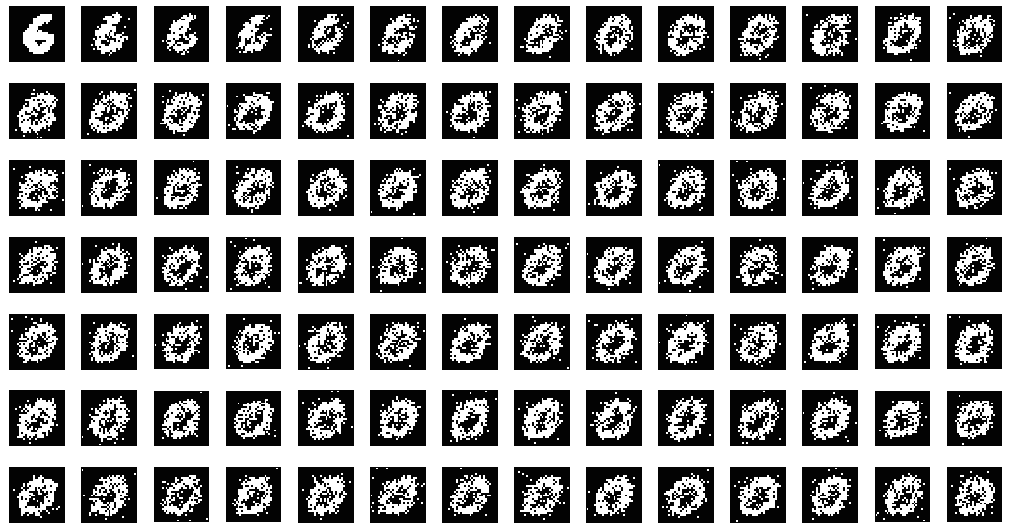
\includegraphics[scale=.3]{../res/chgVisible3.png}
	\caption{The visible neurons at each iteration, (left-to-right, top-to-bottom)}
	\end{minipage}
	\hspace{4em}
	\begin{minipage}[c]{0.35\linewidth}
	\centering
	\vspace{-1em}
	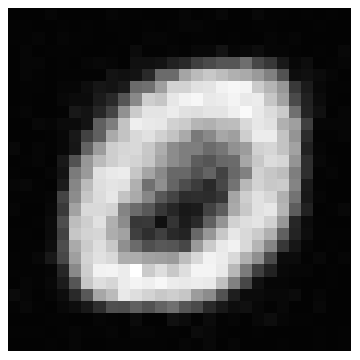
\includegraphics[scale=.45]{../res/avgVisible3.png}
	\caption{Averaged visible neurons}
	\end{minipage}
\end{figure}

\begin{figure}[ht]
	\begin{minipage}[c]{0.5\linewidth}
	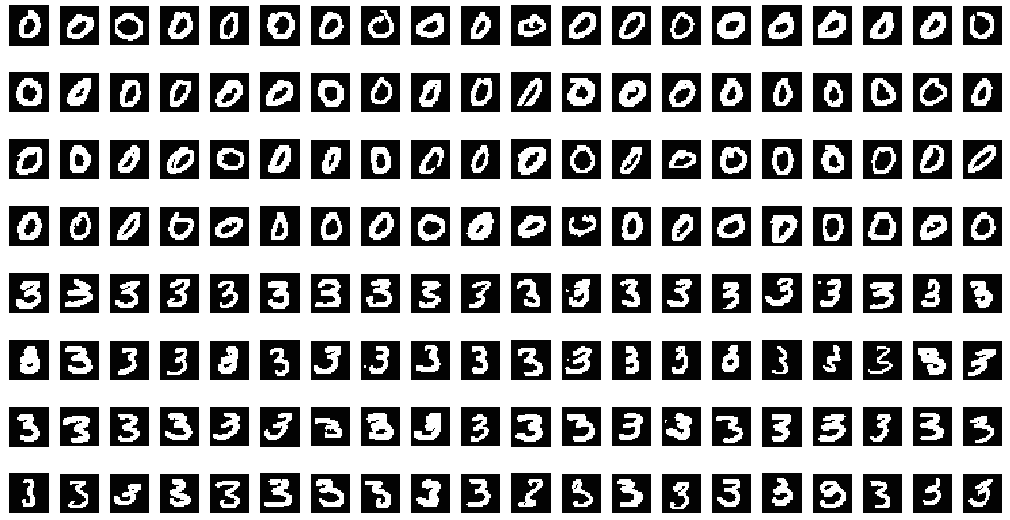
\includegraphics[scale=.25]{../res/testingOrigin0_3.png}
	\end{minipage}
	\begin{minipage}[c]{0.5\linewidth}
	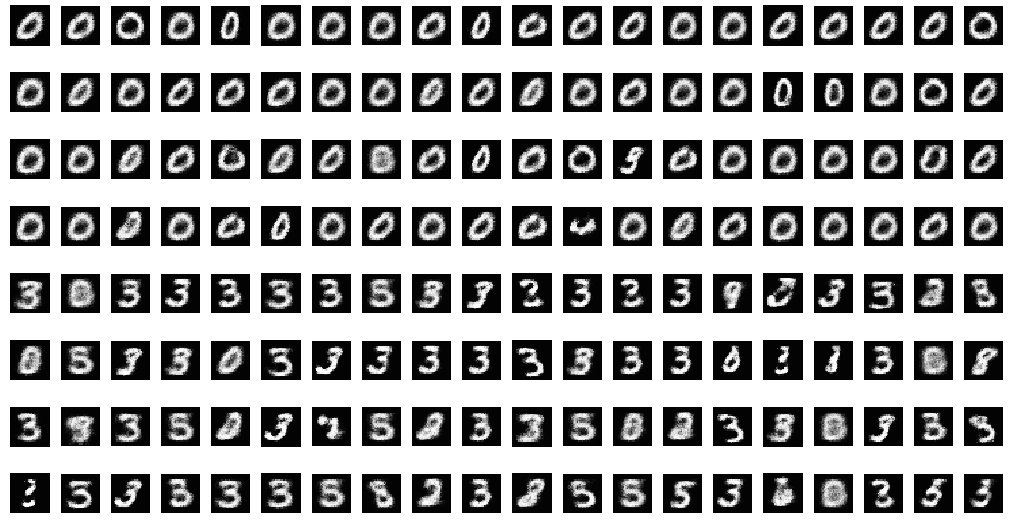
\includegraphics[scale=.25]{../res/testingAvg0_3.png}
	\end{minipage}
	\caption{Better reconstructed results (left: original, right: reconstructed)}
\end{figure}

\begin{figure}[ht]
	\begin{minipage}[c]{0.5\linewidth}
	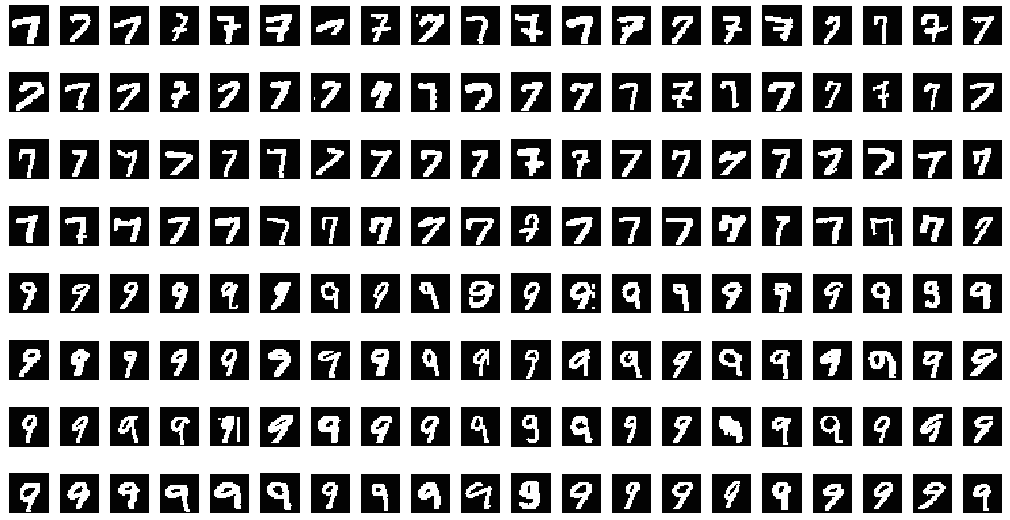
\includegraphics[scale=.25]{../res/testingOrigin7_9.png}
	\end{minipage}
	\begin{minipage}[c]{0.5\linewidth}
	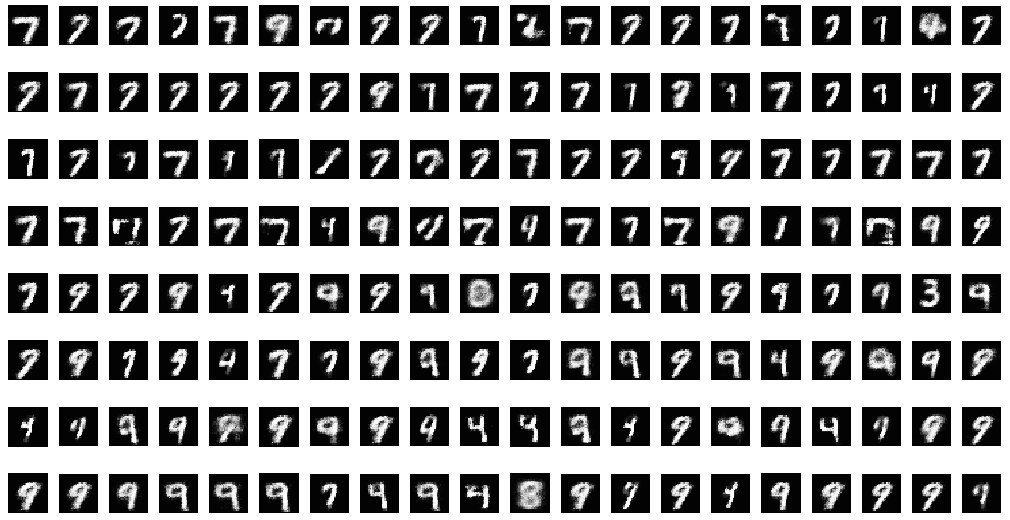
\includegraphics[scale=.25]{../res/testingAvg7_9.png}
	\end{minipage}
	\caption{Worse reconstructed results (left: original, right: reconstructed)}
	\vspace{-3em}
\end{figure}

\newpage
\section*{Discussion}
\vspace{-20pt}
\noindent\makebox[\linewidth]{\rule{\textwidth}{0.4pt}}

\begin{enumerate}
	\item How to initialize the weights?
	\begin{flushleft}
		The weights can not be arbitrarily randomized because every structure has different number of visible/hidden neurons. For adaptivity of any determined structure, I use the strategy that the random variance depends on the number of visible/hidden neurons. In this project, I simply set the variance to $N_v^{-1}$
	\end{flushleft}
	\item How does the learning rate $\eta$ affect the results?
	\begin{flushleft}
		In my experience, different value of learning rate will not affect relative relation between weights in a hidden neuron too much, i.e. a large learning rate can lift weights in a hidden neuron while the ratio between them roughly remains the same, such that they look similar when they are visualized with $\mathsf{imagesc}$ function in MATLAB. As a result, the most critical difference is that the system will get stable more quickly because all weights are at the higher level, such that the probability will be closer to either 1 or 0.
	\end{flushleft}
	\item What have been really learned by the system?
	\begin{flushleft}
		According to the final results shown below, the system seems to learn the shape of digits rather than local features, which is mentioned in the Hinton's lecture.
	\end{flushleft}
	\begin{figure}[ht]
		\hspace{-4.5em}
		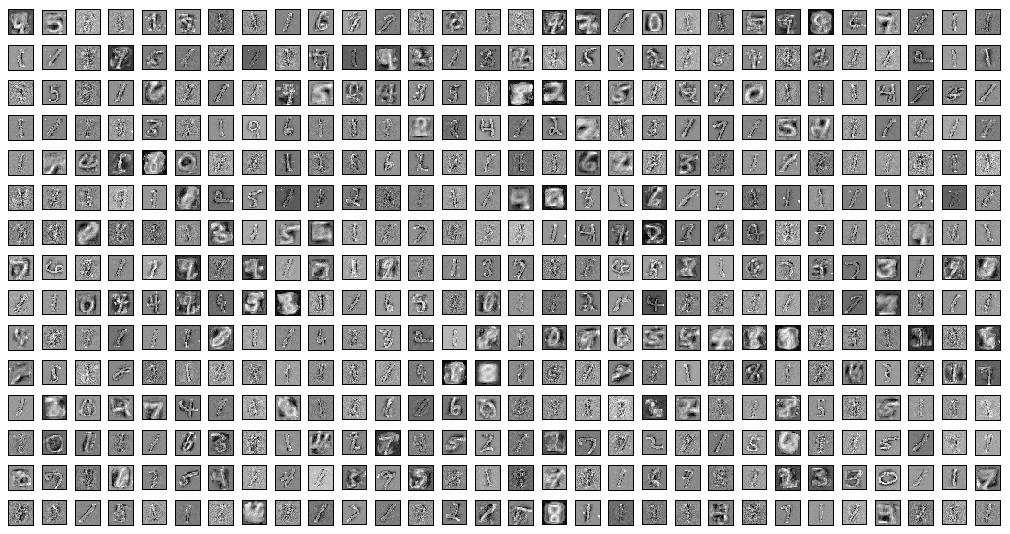
\includegraphics[scale=.6]{../res/weightsAllDigits.png}
		\caption{All final weights}
	\end{figure}
\end{enumerate}

\end{CJK}
\end{document}